% !TEX root = main.tex

\section{Результаты расчётов}

\begin{align*}
    M_{\min} &= 11.74; \\
    M_{\max} &= 18.25; \\
    R &= 6.51; \\
    \hat{\mu}(\vec{X}_n) &= 14.3492; \\
    \sigma^2 &= 1.267; \\
    S^2(\vec{X}_n) &= 1.2776.
\end{align*}

\noindent 
Интервальная групировка значений выборки при $m = 8$:
\[
    [11.74;12.55), [12.55;13.37), [13.37;14.18), [14.18;15.00), [15.00;15.81),
\]
\[
    [15.81;16.62), [16.62;17.44), [17.44;18.25]
\]



\section{Графики}

\subsection{Гистограмма и график функции плотности распределения вероятностей нормальной случайной величины с математическим ожиданием $\hat{\mu}$ и дисперсией $S^2$}


\begin{figure}[h]
    \centering
    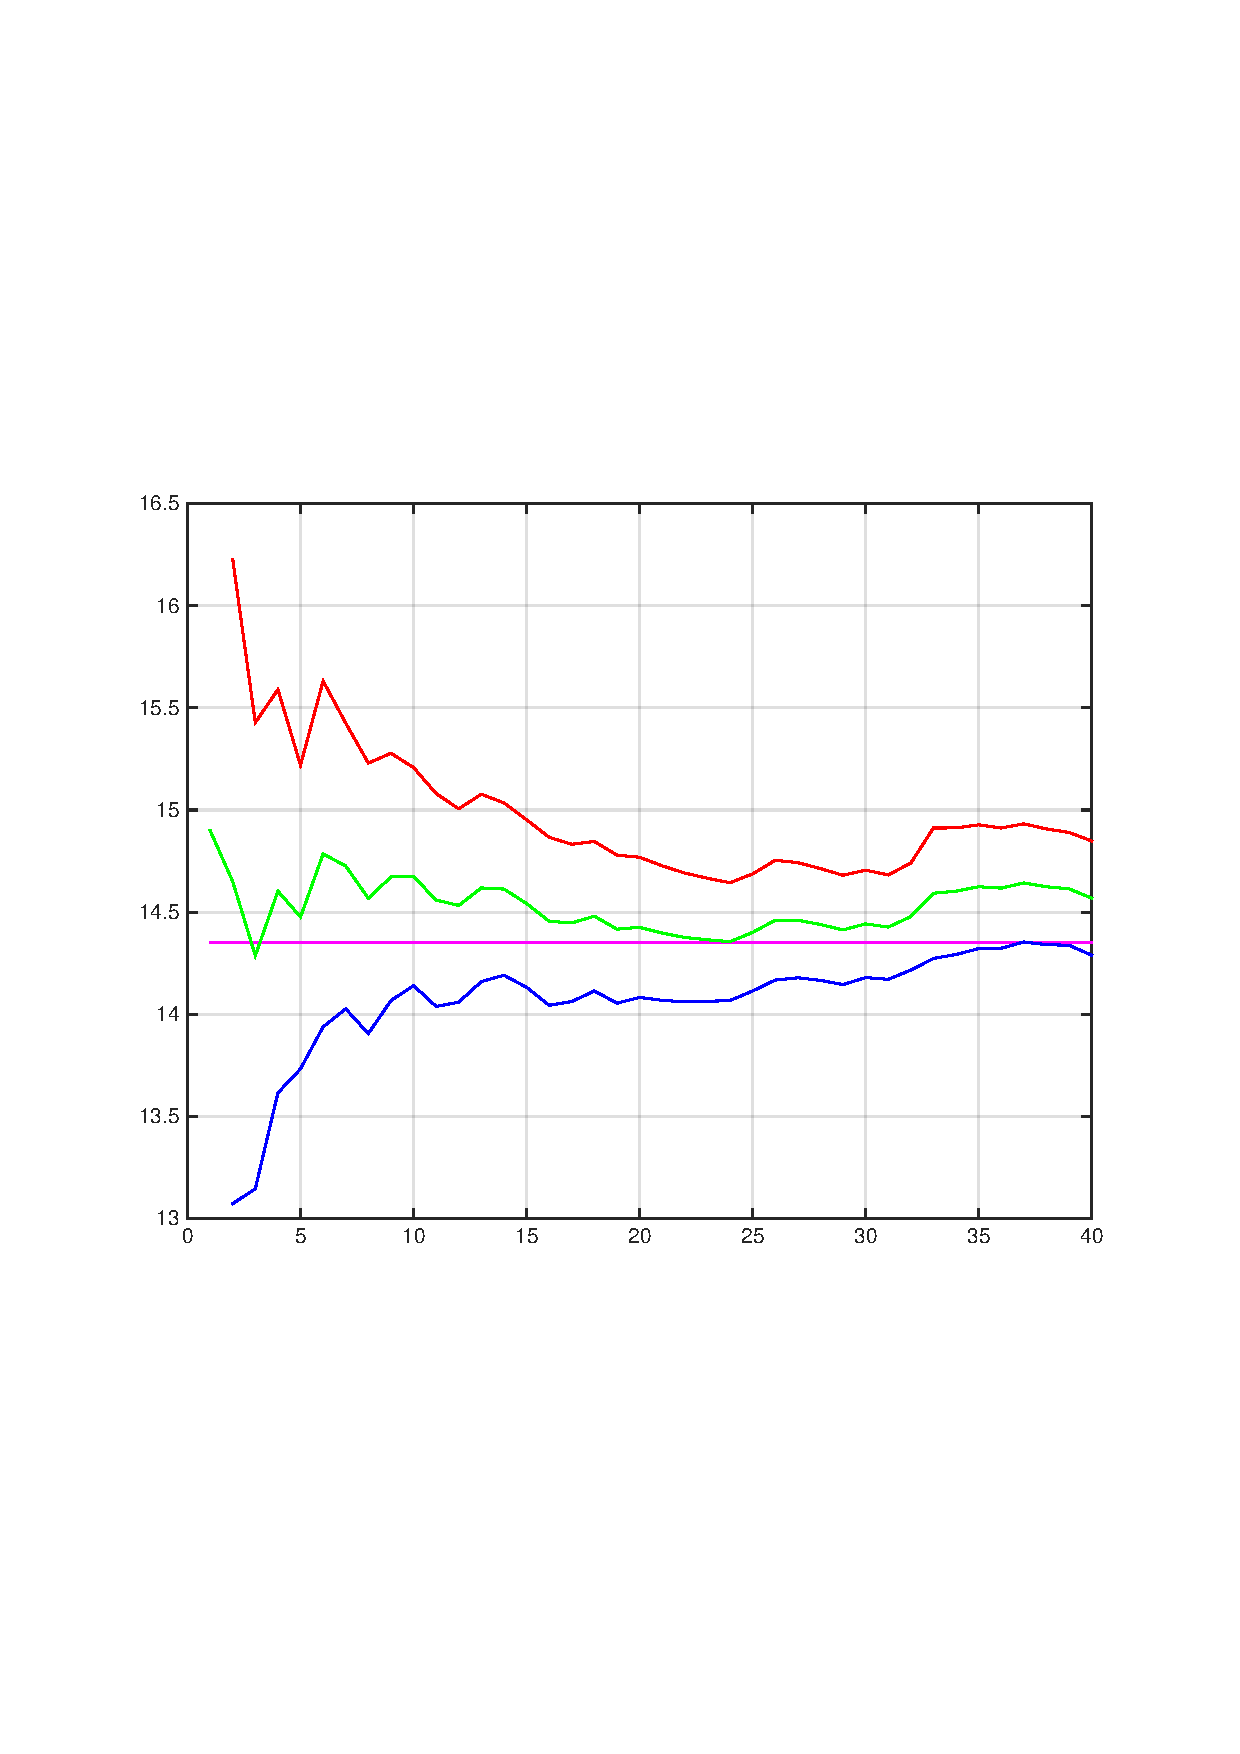
\includegraphics[width=0.7\textwidth]{graphs/figure1.pdf}
    \caption{Гистограмма и график функции плотности распределения нормальной случайной величины.}
\end{figure}



\newpage
\subsection{График эмпирической функции распределения и функции распределения нормальной случайной величины с математическим ожиданием $\hat{\mu}$ и дисперсией $S^2$}

\begin{figure}[h]
    \centering
    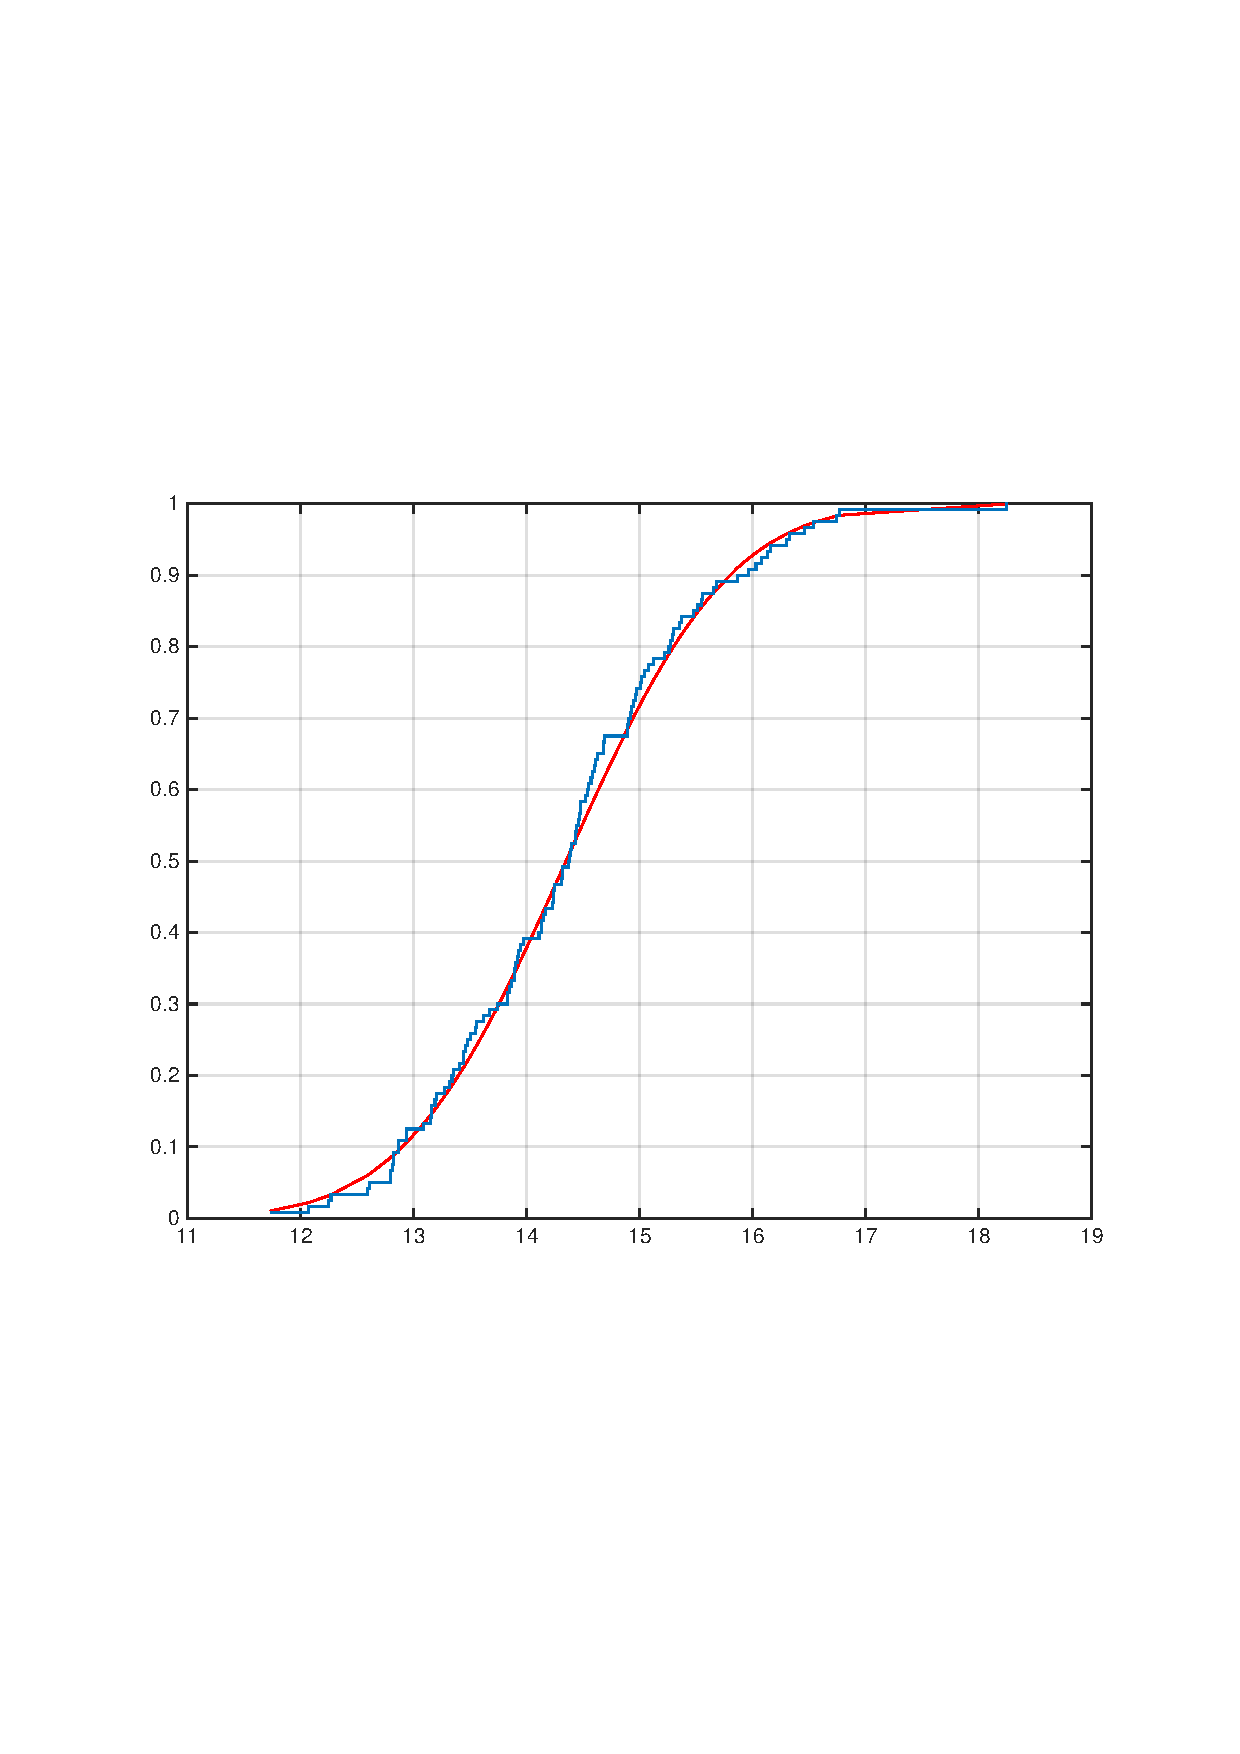
\includegraphics[width=0.7\textwidth]{graphs/figure2.pdf}
    \caption{График эмпирической функции распределения и функции распределения нормальной случайной величины.}
\end{figure}